\documentclass[10pt]{beamer}

\usetheme{CambridgeUS}
\usepackage[english, russian]{babel}
\usepackage[utf8]{inputenc}
\usepackage{caption}
\usepackage{etoolbox}
\usepackage{multicol}
\usepackage{listings}
\usepackage{wasysym}
\usepackage{mathtools}
\DeclarePairedDelimiter\ceil{\lceil}{\rceil}
\DeclarePairedDelimiter\floor{\lfloor}{\rfloor}

\definecolor{mygreen}{rgb}{0,0.6,0}
\lstset{
  basicstyle=\ttfamily\footnotesize,        % the size of the fonts that are used for the code
  breaklines=true,                 % automatic line breaking only at whitespace
  captionpos=b,                    % sets the caption-position to bottom
  commentstyle=\color{mygreen},    % comment style
  keywordstyle=\color{blue},       % keyword style
  stringstyle=\color{red},     % string literal style
  showstringspaces=false,
  morekeywords={include, printf},
  texcl=true     %<---- added
}


\title[\href{https://goo.gl/NRgp8K}{https://goo.gl/NRgp8K} (Term 1)]{Код Хаффмана}
\author[Гусев Илья, Булгаков Илья]{Гусев Илья, Булгаков Илья}
\institute[МФТИ] 
{Московский физико-технический институт\\*}
\date{Москва, 2018}
\subject{Computer Science}

\begin{document}

\begin{frame}
  \titlepage
\end{frame}

\begin{frame}{Содержание}
\tableofcontents
\end{frame}

\section{Коды}
\subsection{Задача}
\begin{frame}[fragile]{Коды}{Задача}
\begin{itemize}
    \item Кодируем последовательность символов битам:
    \begin{itemize}
        \item Без потерь
        \item Однозначно:
        \begin{itemize}
            \item Блочный код (фиксированная длина)
            \item Префиксный код
            \item Постфиксный код
        \end{itemize}
        \item Максимально коротко
    \end{itemize}
\end{itemize}
\end{frame}

\subsection{ASCII}
\begin{frame}[fragile]
\begin{center}
    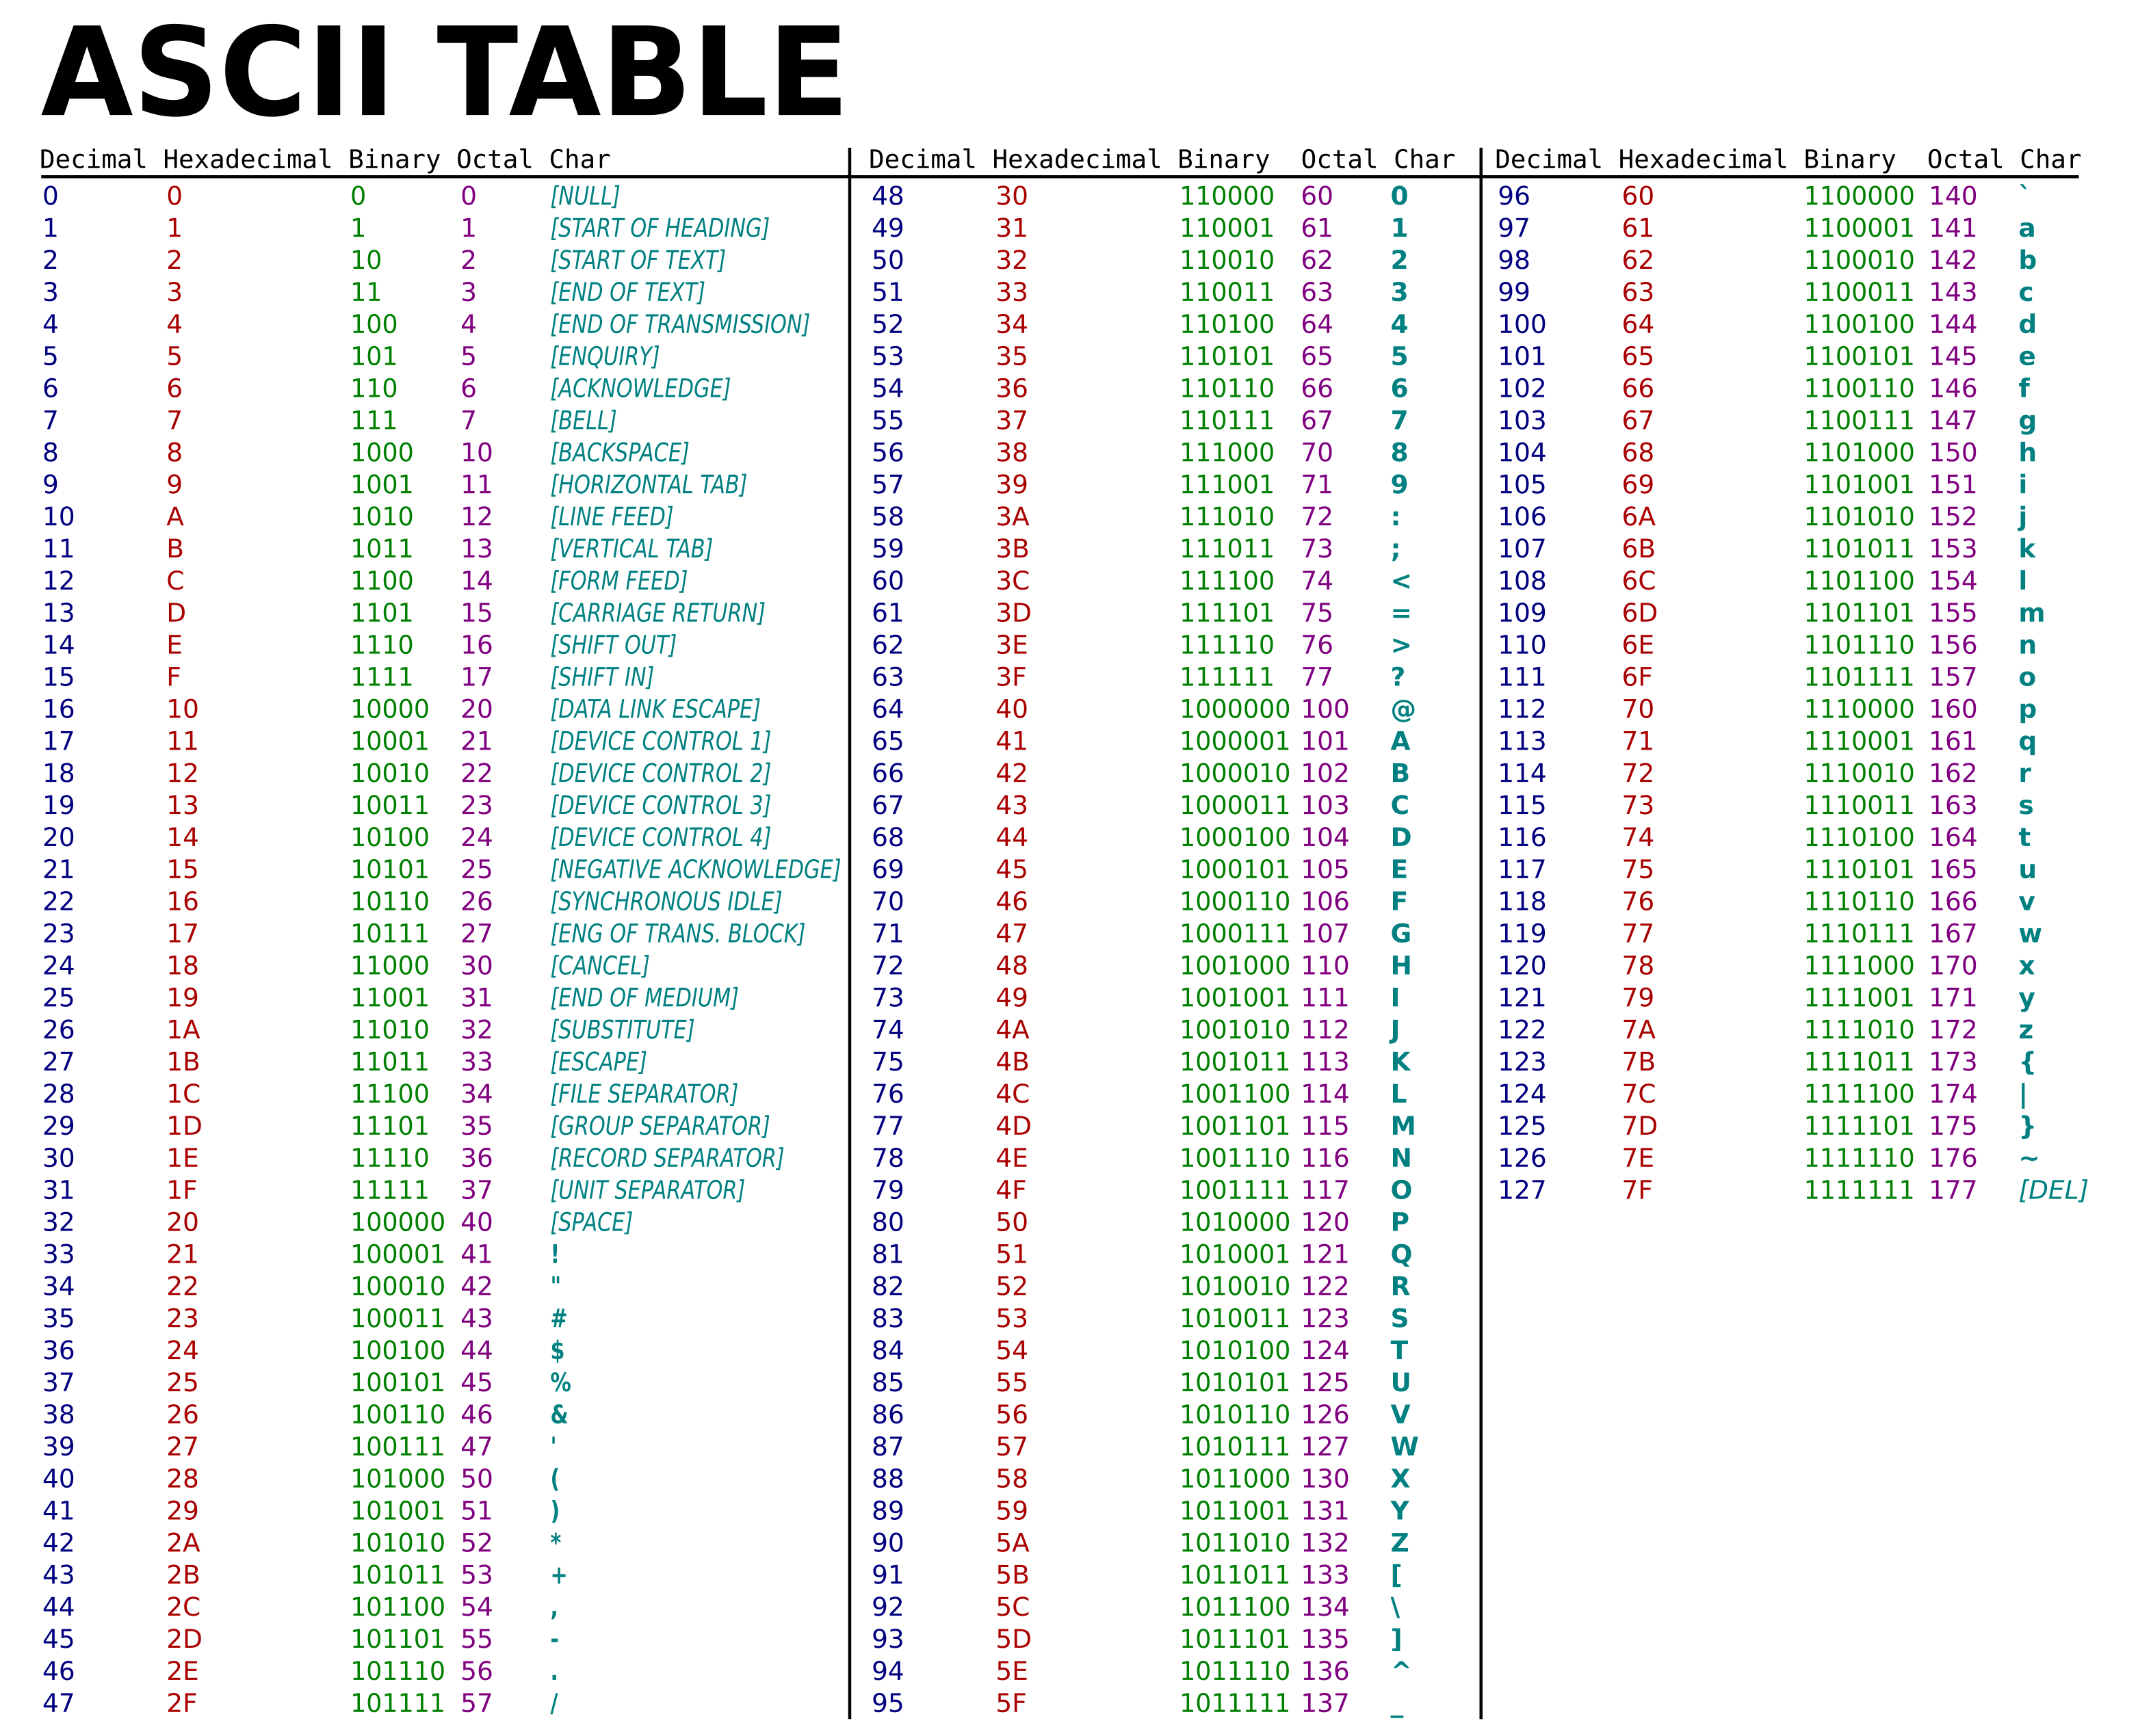
\includegraphics[width=10cm, height=7.7cm]{Term_1/Source/Pirctures/ascii.png}
\end{center}
\end{frame}

\subsection{UTF-8}
\begin{frame}[fragile]{UTF-8}
\begin{itemize}
    \item Фиксированный код переменной длины
    \item Все символы всех живых и мёртвых языков, спец. символы, эмодзи
    \item ASCII-совместима
\end{itemize}
\begin{center}\footnotesize
\begin{tabular}{ |c|c|c|c|c|c|c|c| } 
\hline
Bytes & Bits & First cp & Last cp & Byte 1 & Byte 2 & Byte 3 & Byte 4 \\
\hline
1 & 7 & U+0000 & U+007F & 0xxxxxxx & & & \\
\hline
2 & 11 & U+0080 & U+07FF & 110xxxxx & 10xxxxxx & & \\
\hline
3 & 16 & U+0800 & U+FFFF & 1110xxxx & 10xxxxxx & 10xxxxxx & \\
\hline
4 & 21 & U+10000 & U+10FFFF & 11110xxx & 10xxxxxx & 10xxxxxx & 10xxxxxx \\
\hline
\end{tabular}
\end{center}
\end{frame}

\begin{frame}[fragile]{UTF-8}
\begin{center}
    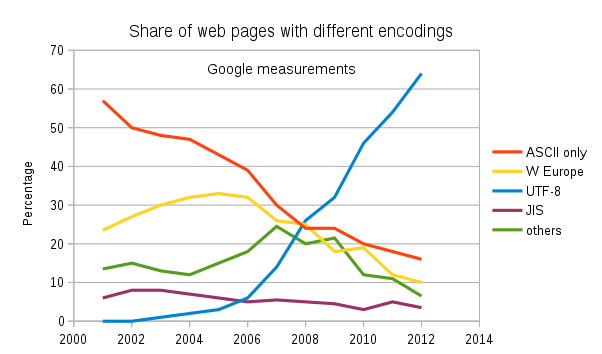
\includegraphics[width=11cm, height=6cm]{Term_1/Source/Pirctures/utf8_growth.png}
\end{center}
\end{frame}

\section{Статический код Хаффмана}
\subsection{Алгоритм}
\begin{frame}[fragile]{Статический код Хаффмана}
\begin{itemize}
    \item Переменная длина, префиксный код
    \item Статичность: заранее считаем частоты символов
    \item Реже встречается символ $\Rightarrow$ больше тратим бит
    \item Используем бинарное дерево
    \item Шаг построения:
    \begin{itemize}
        \item Две наименее частотных вершины подсоединяем к общему родителю
        \item На ребре к меньшей пишем 0, к большей пишем 1
    \end{itemize}
    \item Путь до символа из корня - его код
\end{itemize}
\end{frame}

\begin{frame}[fragile]{Статический код Хаффмана}{Иллюстрация}
\begin{center}
    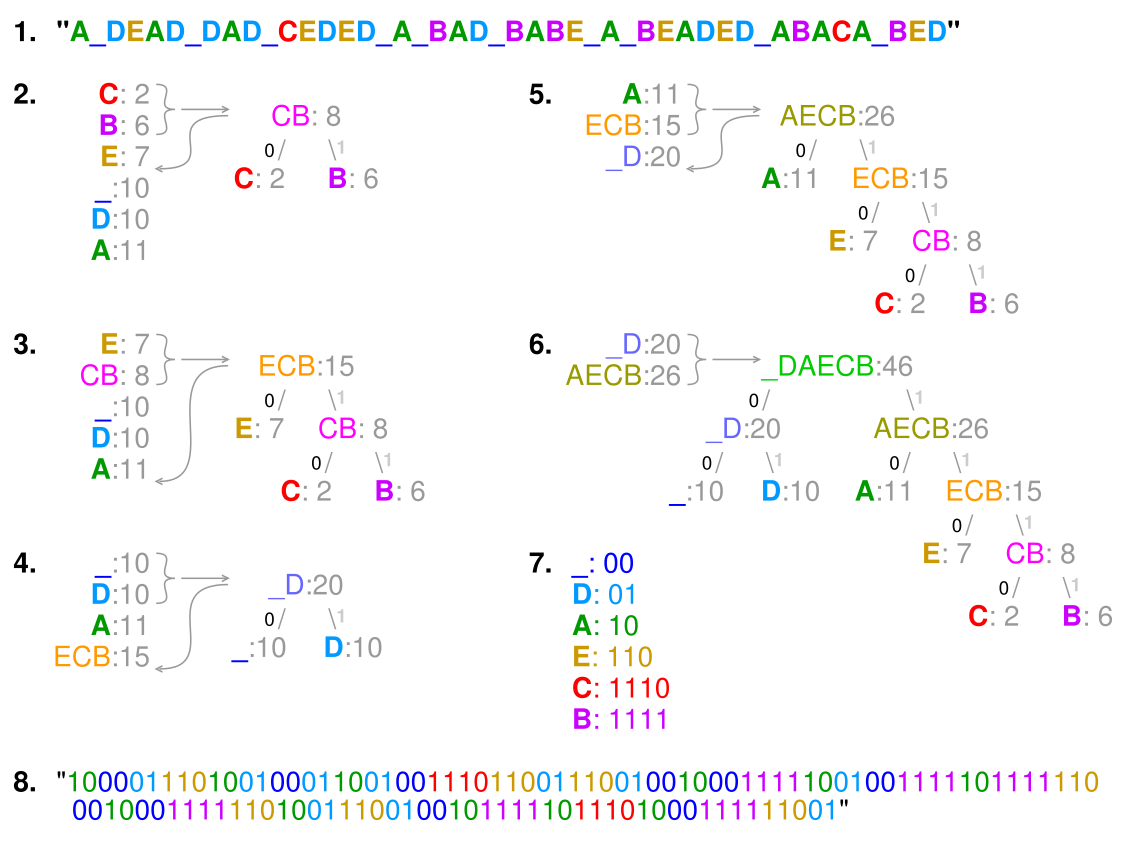
\includegraphics[width=9cm, height=6cm]{Term_1/Source/Pirctures/huffman_big.png}
\end{center}
\end{frame}

\subsection{Особенности}
\begin{frame}[fragile]{Статический код Хаффмана}{Особенности}
\begin{itemize}
    \item Код любого символа не является префиксом любого другого кода
    \item Нужно дописывать таблицу частот в сжатый файл
    \item 2 прохода по сообщению
\end{itemize}
\end{frame}

\section{Адаптивный код Хаффмана}
\subsection{Адаптивность}
\begin{frame}[fragile]{Адаптивный код Хаффмана}{Адаптивность}
\begin{itemize}
    \item Кодируем на ходу
    \item Один проход по сообщению
    \item Не нужно запоминать таблицу символов
\end{itemize}
\end{frame}

\subsection{Реализация}
\begin{frame}[fragile]{Адаптивный код Хаффмана}{Реализация}
\begin{itemize}
    \item Заведём специальный 0-символ с всегда нулевой частотой
    \item Встречаем новый символ $\rightarrow$ пишем 0-символ и сам новый символ
    \item Встречаем старый символ $\rightarrow$ пишем код символа по текущему дереву
    \item Перестраиваем дерево
\end{itemize}
\end{frame}

\subsection{Варианты перестроения дерева}
\begin{frame}[fragile]{Адаптивный код Хаффмана}{Варианты перестроения дерева}
\begin{itemize}
    \item Алгоритм Фоллера, Галлагера, Кнута (ФГК)
    \item Алгоритм Виттера
\end{itemize}
\end{frame}

\section{Бонус}
\begin{frame}[fragile]{Запись битов}
\begin{lstlisting}[language=C++]
std::vector<char> data;
int lastBitsCount = 0;

void WriteBit(bool bit)
{
    if(lastBitsCount == 0) {
        data.push_back(0);
    }
    if(bit) {
        data.back() |= 1 << lastBitsCount;
    }
    lastBitsCount = (lastBitsCount + 1) % 8;
}
 
void WriteByte(char value)
{
    for( int i = 0; i < 8; ++i ) {
        WriteBit((value & (1 << i)) != 0);
    }
}
\end{lstlisting}
\end{frame}


\appendix
\section<presentation>*{\appendixname}
\subsection<presentation>*{Useful links}

\begin{frame}[allowframebreaks]
  \frametitle<presentation>{Полезные ссылки}
    
  \begin{thebibliography}{10}
{
  \beamertemplatearticlebibitems
  \bibitem{wiki_unicode}
  \texttt{Вики: Юникод}
  \newblock \href{https://ru.wikipedia.org/wiki/\%D0\%AE\%D0\%BD\%D0\%B8\%D0\%BA\%D0\%BE\%D0\%B4}{\texttt{https://ru.wikipedia.org/wiki/Юникод
}}
  
  \bibitem{wiki1}
  \texttt{Wiki: Huffman coding}
  \newblock \href{https://en.wikipedia.org/wiki/Huffman_coding}{\texttt{https://en.wikipedia.org/wiki/Huffman\_coding}}
  
  \bibitem{wiki2}
  \texttt{Вики: Адаптивный алгоритм Хаффмана}
  \newblock \href{https://bit.ly/2DBDFoA}{\texttt{https://bit.ly/2DBDFoA}}
  
  \bibitem{wiki3}
  \texttt{Викиконспекты: Алгоритм Хаффмана за O(n)}
  \newblock \href{https://bit.ly/2qFhK7B}{\texttt{https://bit.ly/2qFhK7B}}
  
  \bibitem{cru}
  \texttt{Compression.ru: Динамическое сжатие методом Хаффмана}
  \newblock \href{https://bit.ly/2Dy4Dxp}{\texttt{https://bit.ly/2Dy4Dxp}}

}


  \end{thebibliography}
\end{frame}

\end{document}


